
\let\negmedspace\undefined
\let\negthickspace\undefined
\documentclass[journal]{IEEEtran}
\usepackage[a5paper, margin=10mm, onecolumn]{geometry}
%\usepackage{lmodern} % Ensure lmodern is loaded for pdflatex
\usepackage{tfrupee} % Include tfrupee package
\setlength{\headheight}{1cm} % Set the height of the header box
\setlength{\headsep}{0mm}     % Set the distance between the header box and the top of the text
\usepackage{gvv-book}
\usepackage{gvv}
\usepackage{cite}
\usepackage{amsmath,amssymb,amsfonts,amsthm}
\usepackage{algorithmic}
\usepackage{graphicx}
\usepackage{textcomp}
\usepackage{xcolor}
\usepackage{txfonts}
\usepackage{listings}
\usepackage{enumitem}
\usepackage{mathtools}
\usepackage{gensymb}
\usepackage{comment}
\usepackage[breaklinks=true]{hyperref}
\usepackage{tkz-euclide} 
\usepackage{listings}
% \usepackage{gvv}                                        
\def\inputGnumericTable{}                                 
\usepackage[latin1]{inputenc}                                
\usepackage{color}                                            
\usepackage{array}                                            
\usepackage{longtable}                                       
\usepackage{calc}                                             
\usepackage{multirow}                                         
\usepackage{hhline}                                           
\usepackage{ifthen}                                           
\usepackage{lscape}
\renewcommand{\thefigure}{\theenumi}
\renewcommand{\thetable}{\theenumi}
\setlength{\intextsep}{10pt} % Space between text and floats
\numberwithin{equation}{enumi}
\numberwithin{figure}{enumi}
\renewcommand{\thetable}{\theenumi}
\begin{document}
\bibliographystyle{IEEEtran}
\title{Question 9-9.3-11}
\author{EE24BTECH11041 - Mohit}
% \maketitle
% \newpage
% \bigskip
{\let\newpage\relax\maketitle}
\begin{enumerate}
\item 
If the area of the region bounded by the line $y=mx+c$ and the curve $x^2=y$ is $\frac{32}{7}$sq.unit then find the positive value of $m$.
\end{enumerate}
\begin{table}[h!]    
  \centering
  \begin{tabular}[12pt]{ |c| c|}
    \hline
    \textbf{Variable} & \textbf{Description} \\ 
    \hline
    $\vec{x_1}$ & Point on circle \\
    \hline
    $\vec{x_2}$ & Point on circle \\
    \hline 
    $\vec{n}$ &  Equation of line on centre of circle lies \\
    \hline   
    \end{tabular}

  \caption{Variables Used}
  \label{tab 1.4.9.2}
\end{table}
	
The parameters of the given conic are
\begin{align}
\vec{V}=\myvec{
1 & 0\\
0 & 0
},
\vec{u}=\myvec{0\\-\frac{1}{2}},
f=0.
\end{align} 
For the line, the parameters are
\begin{align}
\vec{h} = \myvec{
0\\
c
},
\vec{m} = \myvec{1 \\ m}
\end{align}
x-coordinate of point of intersection are 
\begin{align}
    x_1=\frac{m-\sqrt{m^2+4c}}{2},x_2=\frac{m+\sqrt{m^2+4c}}{2}
\end{align}
From the desired area is 
\begin{align}
\vec{A}=\int_{x_1}^{x_2} (mx+c-x^2) \,dx = \frac{m}{2}(x_2^2-x_1^2) + c(x_2-x_1) -\frac{1}{3}(x_2^3 - x_1^3) = 32/7
\end{align}
On solving,we get m=2.86 and c=2
 
Hence, the slop line is 2.86.
\begin{figure}[h!]
   \centering
   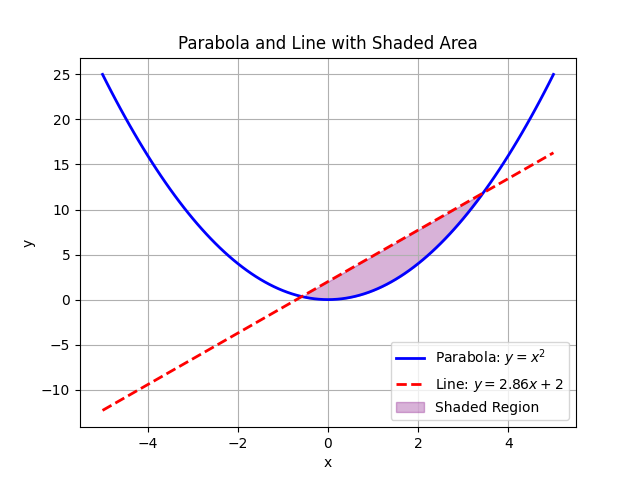
\includegraphics[width=0.7\linewidth]{figs/Figure_1.png}
   \caption{Plot of curves}
   \label{stemplot}
\end{figure}
\end{document}
